%======================================================================
\chapter{Video Object Segmentation}
\label{chap:vos}
%======================================================================

In this section, we present a method for extracting foreground objects from video and its application to content-aware video compression. Our method uses trimaps inferred from background subtraction to represent the foreground-background relationship. The appearance of foreground and background are modelled with Radial Basis Functions initialized from the background substraction step. Finally, Graph Cuts are used to compute a binary mask. Our method is fully automatic, fast, and does not make restrictive assumptions about object motions. In experiments on standard data sets, the proposed approach achieves comparable results to state-of-the-art video object segmentation methods but our method is much faster. We also demonstrate an application of the proposed method to content-aware video compression.

\section{Introduction}
\label{sec:vos:i}

Video object segmentation is the process of separating foreground objects from the background in a video~\cite{papazoglou2013}. A wide range of applications benefit from the progress of video object segmentation, e.g. robot-object interaction, recognition, and video compression.

A variety of methods have been proposed to address the task~\cite{papazoglou2013,ma2012,wang2015,brox2010,taylor2015}. Most methods use motion cues to initialize the object segmentation.
A common method for motion detection is  background subtraction with mixture of Gaussians~\cite{kaewtrakulpong2002,zivkovic2004}. This technique models each pixel indepedently as a mixture of Gaussians, but as it detects motion in each frame independently, the results lack completeness and temporal persistence.
In this paper, we address this shortcoming by modelling the appearance of objects from motion. 

Our proposed method treats moving pixels as a partial segmentation of objects and builds the appearance model for them, see Section~\ref{sec:vos:m:csc}. With the appearance model, those pixels that are not moving can successfully be classified as foreground or background to form a more complete segmentation. We model appearance with Radial Basis Functions (RBF) as described in Section~\ref{sec:vos:m:csc}, an approach commonly used in interactive editing for selection propagation~\cite{li2010,tao2012}. We adapt the technique of Tao and Krishnaswamy~\cite{tao2012} but use motion detection instead of user selection to initialize the models.
 
Moving pixels obtained with background subtraction approaches may be not just incomplete, but also contain pixels from the background. This is mainly caused by shadows and noise. The consequence is that the computed segmentations are likely to cover regions that are not part of the foreground. We address this mis-classification with modelling background appearance and optimizing the classification. We use Graph Cuts~\cite{greig1989,boykov2004} to optimize the foreground and background classification based on the appearance model. To accelerate the computation, we divide frames into regions that contain one object each (see Section~\ref{sec:vos:m:tg}), and oversegment those regions with a fast superpixel method~\cite{siva2014} before classification (see Section~\ref{sec:vos:m:fbl}).

We evaluate our video object segmentation approach on a common dataset~\cite{f-li2013} in Section~\ref{sec:vos:e:ds}. Our evaluation demonstrates that our approach achieves comparable results to two state-of-the-art approaches, but our approach is on-line and is $10-200 \times$ faster than these methods.

The major contribution of our work is a fast on-line video object segmentation method that takes both motion and appearance of objects into account. We propose a novel integration of RBF appearance modelling and background subtraction through a Graph Cuts optimization on superpixels. We use local modelling to accelerate segmentation by dividing frames into regions that contain one foreground object each which greatly reduces the number of pixels to be processed. In Section~\ref{sec:vos:cavc}, we propose an application of our on-line approach for compressing videos with compression quality adapted to foreground and background. The video object segmentation allows us to reduce the quality of the background by pre-processing it with a bilateral filter before compression while foreground objects are compressed as is by the compression scheme. We use H.264 coding.

\section{Background}
\label{sec:vos:bg}

A large number of methods have been proposed for extracting moving objects from an image sequence, using motion, depth, appearance, or a combination of these cues.
Among those, motion is used most frequently as cues for object extraction~\cite{graciela2013}, and many approaches use
background subtraction to this end~\cite{zeng2007,colombari2007}.
Classic background subtraction methods model the appearance of the background at each pixel and label the pixel that change rapidly to be foreground~\cite{jain1979,kaewtrakulpong2002,zivkovic2004}. These methods typically assume a stationary or slowly panning camera.
More recently, optical flow is also used~\cite{ma2012,papazoglou2013,zhang2013,wang2015}.
The motion estimation algorithms typically provide pixel-wise labeling and errors are inevitable even when using state-of-art algorithms.
To obtain robuster masks with semantic meaning, energy minimization is often used~\cite{papazoglou2013}.
Optical flow usually provides more motion cues than background subtraction (e.g. pixel correspondence across frames), but in general, is much slower than background subtraction methods.
Our approach is closely related to tracking. We infer trimaps from detected motion to coarsely separate foreground from background, which is different from other methods based on motion cues~\cite{papazoglou2013,wang2015}.

With the advances in computational power of modern PCs and the progress of fast superpixel methods, the use of superpixels as units of object extraction is increasingly becoming popular~\cite{papazoglou2013,wang2015,ochs2011}. Instead of naive superpixel voting schemes, researchers often use some optimization approaches to decide if a superpixel belongs to the foreground or the background~\cite{papazoglou2013,wang2015,ochs2011}. However, most of the superpixel methods are computationally intensive, which prevents their use in real-time video object extraction~\cite{achanta2012}. A fast superpixel method was proposed by Siva and Wang~\cite{siva2014}. It is based on seam carving and dynamic programming, and it achieves real-time performance in low resolution videos. We adapt this method and further accelerate the computation of superpixels by only segmenting the regions within the bounding boxes of foreground objects into superpixels.

Several video object extraction methods track points over the image sequences and then cluster the resulting point trajectories pairwise or in triplets~\cite{brox2010,ochs2011,ochs2012}.
The advantage of employing point tracking is the capacity of handling videos where moving objects are stationary in a number of frames.
The underlying assumption induced is that the objects are rigid so that all object points move according to a single translation~\cite{brox2010,ochs2011}, while the work of Ochs et al.~\cite{ochs2012} assumes a single similarity transformation. This assumption makes these methods not applicable to non-rigid objects.
The methods produce a sparse labeling in each frame, and superpixels are taken into account when turning the point trajectories into dense regions.
These methods are also able to handle partial occlusion but the drawback is that they are very slow (in the order of minutes per frame).

The work by Lee et al.~\cite{lee2011} shows the potential of using shape matching in object extraction.
The method first identifies object-like regions in any frame~\cite{endres2010}, followed by computing a series of binary partitions among those candidate regions to discover groups of shapes with persistent appearance and motion.
The drawbacks of this method include that it requires pre-processing identifying all object-like regions beforehand, it is very slow (in the order of minutes per frame), and it is not applicable to stationary or occluded (in some frames) foreground objects.

Depth information has been demonstrated to be robust to environment changes such as illumination change, dynamic backgrounds, and camera motion~\cite{dahan2011,taylor2015}.
The work of Taylor et al.~\cite{taylor2015} infers depth layers from occlusion information. This gives it the capacity to be used outdoors and ensures that it is robust to occlusion and disocclusion. However, the method takes around 30 seconds for a VGA image on a standard desktop.

The works of Papazoglou and Ferrari~\cite{papazoglou2013} and Wang et al.~\cite{wang2015} are closely related to ours. Papazoglou and Ferrari~\cite{papazoglou2013} use optical flow as the motion cues. After generating a coarse segmentation, Graph Cuts are used to minimize an energy function containing an appearance term and smoothness terms. In this paper, we propose a novel algorithm based on Radial Basis Functions to model the appearance and estimate how close it is from a pixel to foreground or background, considering the neighbouring frames. We also use Graph Cuts to obtain the final masks.

Many modern approaches offer offline processing to recognize objects in videos~\cite{papazoglou2013,ma2012,wang2015,brox2010}. The requirement of the availability of the entire video limits those methods in processing long sequences.
In contrast, our method is online and offers processing in "streaming", which gives it the capacity to handle longer videos and integrate with other online applications.

\section{Method}
\label{sec:vos:m}

Our method consists of three steps: (1) trimap generation, (2) color similarity calculation, (3) foreground-background labelling. Figure~\ref{fig-overview} illustrates the overview of the proposed pipeline. First, motion is detected with the background subtraction method, followed by blob analysis to generate trimaps. Second, the appearance model is built with Radial Basis Functions, where sampling is done in different regions of the trimap for foreground and background respectively. With knowing how close a pixel is to the foreground or the background according to its color, we produce evidence maps. To enhance the spatial and temporal persistency, we smooth the maps with a bilateral filter kernel. Third, using Graph Cuts, we are able to generate a binary mask by minimizing an energy function. Next, we present the detail of these steps.

\begin{figure*}
	\centering
	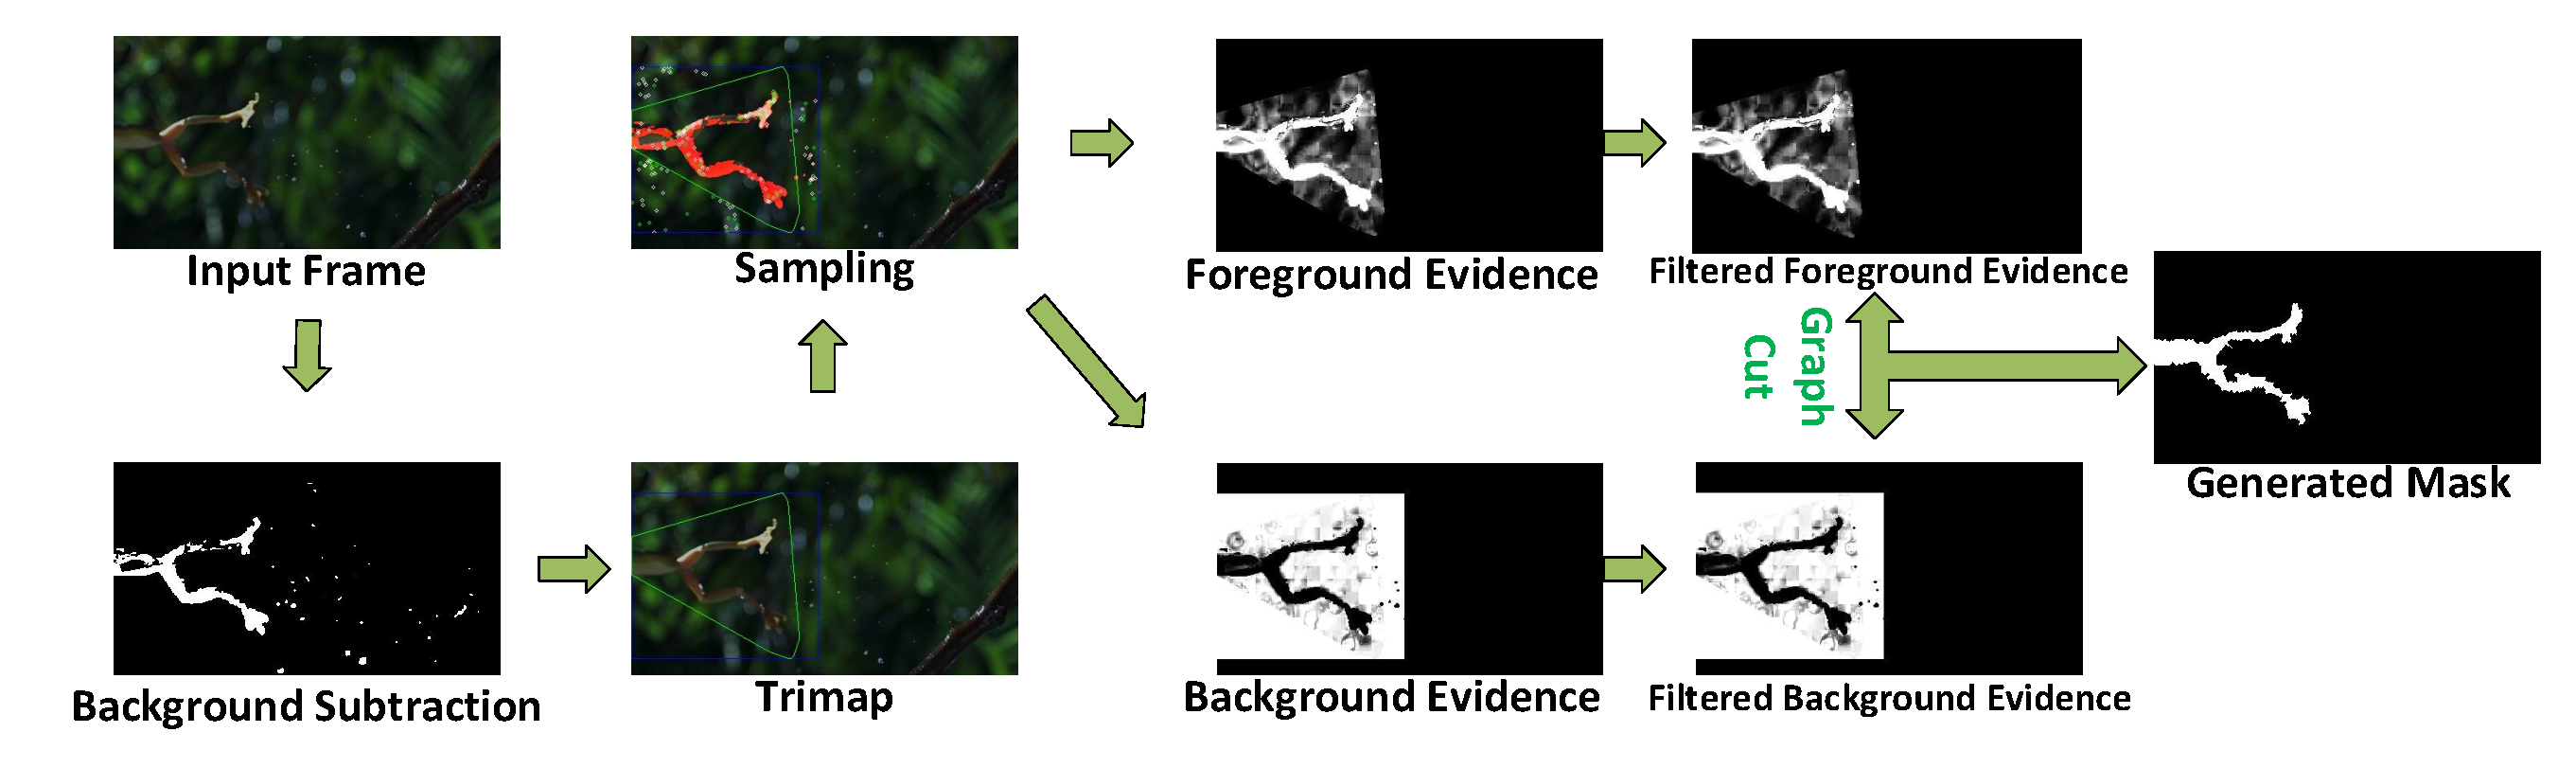
\includegraphics[width=\textwidth]{figures/overview.pdf}
	\caption{Overview of the proposed video object segmentation method. The images are a frame from the dataset SegTrack v2~\cite{f-li2013}.}
	\label{fig-overview}
\end{figure*}

\subsection{Trimap Generation}
\label{sec:vos:m:tg}

\textbf{Background subtraction.}
We begin by computing background subtraction frame by frame using effective  mixture of Gaussians algorithms~\cite{kaewtrakulpong2002,zivkovic2004} according to a comparison~\cite{sobral2014} of various background subtraction methods. We employ the implementations of the two algorithms MOG and MOG2 in OpenCV. After background subtraction, we perform a median filter of kernel size 3 to reduce noise, see Figure~\ref{fig-trimap}(b).

\textbf{Blob analysis.}
After obtaining moving pixels in the background subtraction step, we apply closing morphological transformation to group them. We perform a dilation step followed by an erosion in the binary labelling of the image as it is typically used to close small hole inside the foreground objects.
The purpose of grouping moving pixels is to reduce isolated moving pixels.
Then the convex hulls of blob contours are calculated. The contours are found using Suzuki's algorithm~\cite{suzuki1985} while convex hulls are calculated using Sklansky's algorithm~\cite{sklansky1982}. The bounding boxes are then computed from the convex hulls, see Figure \ref{fig-trimap}(c).

We base our trimap generation on the contours and bounding boxes of the blobs of moving pixels.
A trimap is a partition of images into three regions: a definite foreground, a definite background, and a blended region where pixels are considered as a mixture of foreground and background colors.
More specifically, moving pixels obtained using background subtraction serve as the definite foreground, while the pixels inside the bounding box and outside of the convex hull are treated as definite background.
Those pixels inside the convex hull but not recognized as moving pixels are the blended region.
Such a trimap is established for each blob and segmented individually.
Because in some cases, background subtraction generates trimaps smaller than the actual size of objects, we expand the areas of the convex hulls and bounding boxes by a ratio $r$ such that $A^{*}=r\cdot A$, where $A$ and $A^{*}$ are the areas before and after expansion respectively, see Figure~\ref{fig-trimap}(d).  In our implementation, we typically use $r=2$.

\begin{figure}
	\centering
	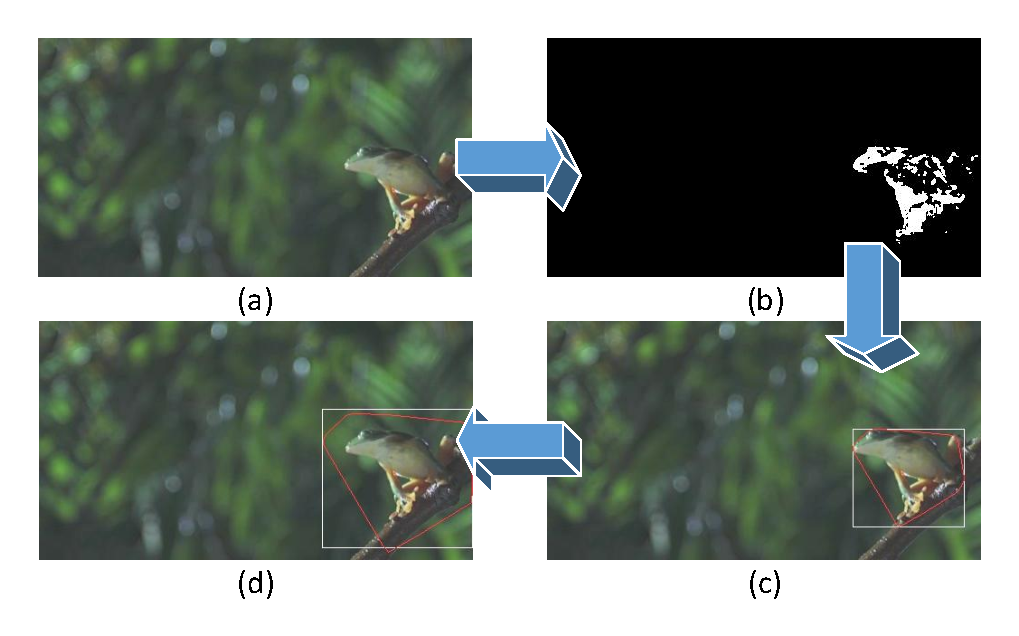
\includegraphics[width=3.3in]{figures/trimap.pdf}
	\caption{Trimap generation. (a) Original frame. (b) Background subtraction result. (c) Convex hull (red) and bounding box (white) of the blob. (d) Convex hull (red) and bounding box (white) after expansion. The images are a frame from the dataset SegTrack v2~\cite{f-li2013}.}
	\label{fig-trimap}
\end{figure}

\subsection{Color Similarity Calculation}
\label{sec:vos:m:csc}

The goal of this stage is to estimate the distance of a pixel to the foreground and the background based on a color similarity metric between every pixel in the blended region and the definite regions.

\textbf{Radial Basis Functions}
Li et al.\ described in detail a method using Radial Basis Functions (RBF) to propagate user edits in image matting \cite{li2010}.
Similar to \cite{li2010}, we use RBF to account for all the pixels within the definite foreground or the background regions.
However, we define the RBF in the three-dimensional color space where each pixel $i$ is represented by its feature vector $\mathbf{f}_{i}$.
The method samples the foreground pixels and the background pixels, respectively, and computes the coefficients of the Radial Basis Functions subject to interpolation constraints using a linear solver.
With $G$ representing all foreground or background pixels, we formulate the interpolation constraints as a least-square energy function, 
\begin{equation}
\label{equ-rbf-ef}
\sum_{i\in E}{(1-h(\mathbf{f}_{i}))^2}
\end{equation}
where $E\in G$ is the subset of all definite foreground or background pixels, and $\mathbf{f}_{i}$ is the color vector of pixel $i$.
$h(\cdot)$ is the RBF centered at the pixels in $B\in G$, where $B$ is another subset of $G$.
To allow {\em soft} interpolation and to gain computational efficiency, we define that $|B| < |E|$, where $|\cdot|$ counts the number of pixels in a set. We choose to sample the set $E$ to have twice the size of $B$. Let
\begin{eqnarray}
\label{equ-rbf}
h(\mathbf{f})&=&\sum_{i\in B}{a_{i}\phi(||\mathbf{f}-\mathbf{f}_{i}||)} \\
\mbox{with}\;\;
% \label{equ-basis}
\phi(r)&=&exp(-\sigma *r^2) \nonumber
\end{eqnarray}
where $\mathbf{f}$ is any point in the color space, $a_{i}$ are the unknown coefficients, $\phi(\cdot)$ is some pre-defined radial basis, and $\sigma$ controls the smoothness of the Gaussian bases~\cite{li2010}.

The coefficients $a_{i}$ represent the importance of a color being similar to a color within the set $B$. Equation~\ref{equ-rbf} directly estimates the similarity of a color to all the colors in the foreground or the background regions. Pixels with the value of 1 are most similar to the corresponding definite region while pixels with the value of 0 represent dissimilar colors. As subsets are sampled from definite regions and Equation~\ref{equ-rbf-ef} is over-determined, the values of pixels may be greater than 1 or less than 0, but we clip the values to $[0,1]$.

The reason why we use a subset $E\in G$ instead of $G$ to construct Equation~\ref{equ-rbf-ef} is to accelerate the computation because each pixel is costly due to the use of the linear solver to compute the RBF~\cite{tao2012}.
%With high-resolution videos, the number of pixels in $G$ can be large, and there is no need to use all pixels in foreground and background regions, respectively, as long as consistent results can be maintained. With too few samples, the RBF behaves inconsistently and sampling plays a critical role in determining the quality of the function. As discussed by Tao and Krishnaswamy~\cite{tao2012}, if pixels are sampled randomly, noise affects the results. Figure \ref{fig-image-matting} shows an example of computing color similarity with RBF.

\begin{figure}
	\centering
	\subfigure[Input Image and Strokes]{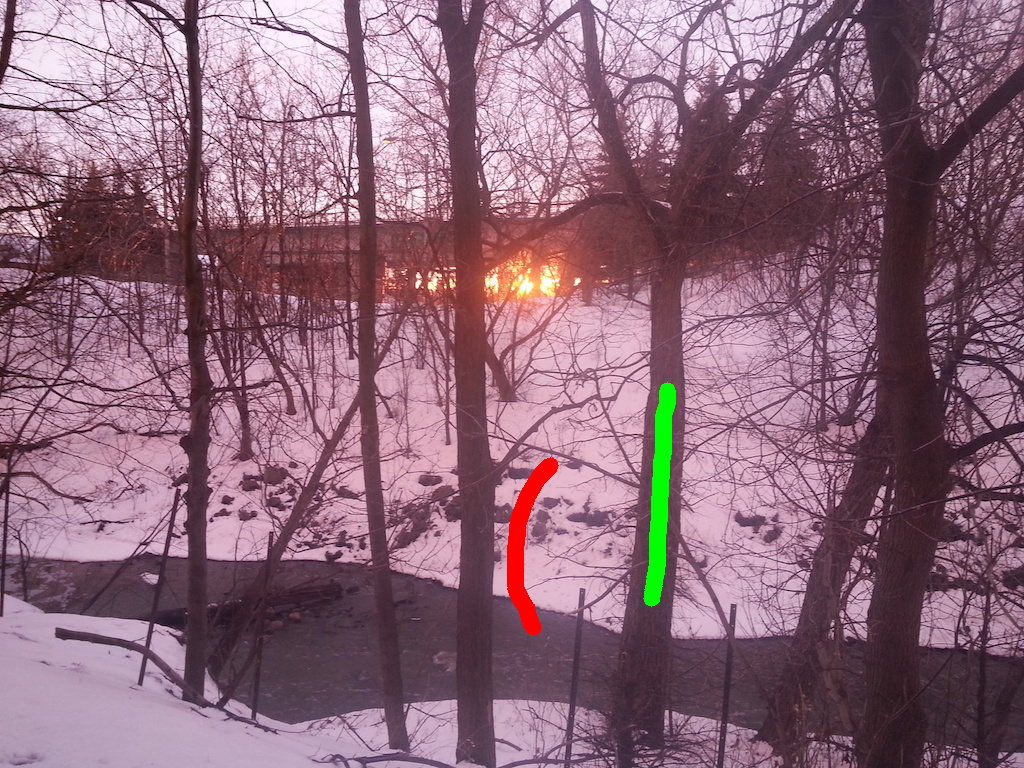
\includegraphics[width=0.35\columnwidth]{figures/img_selects.png}}
	\subfigure[Output Image]{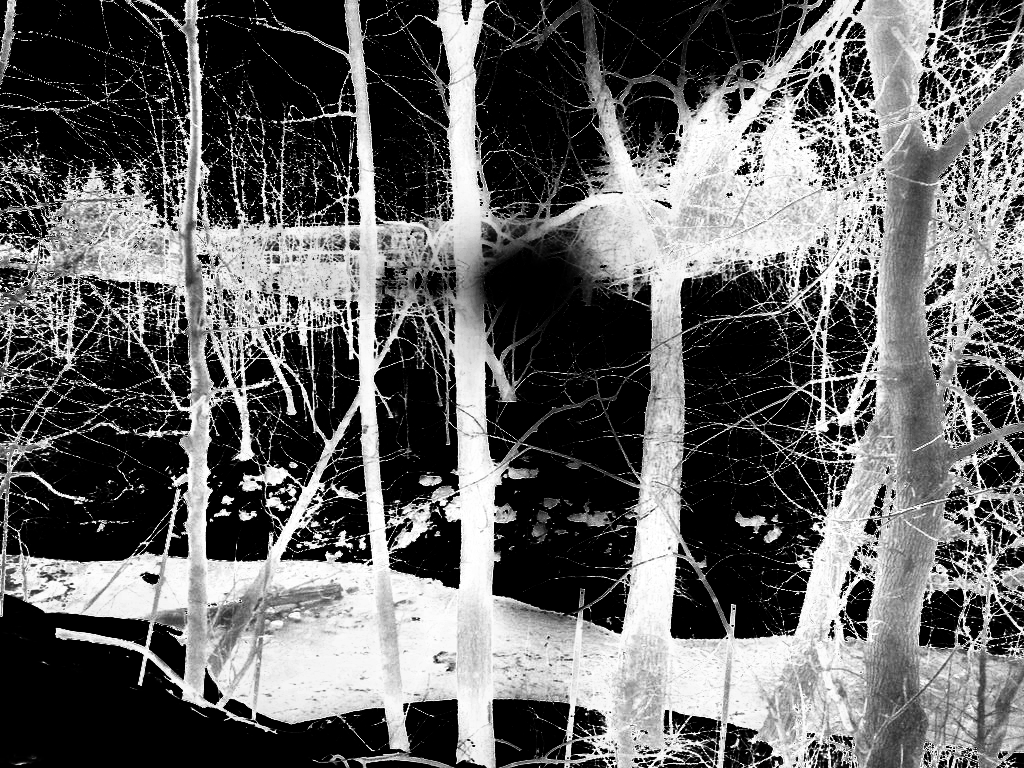
\includegraphics[width=0.35\columnwidth]{figures/sMap.png}}
	\caption{An example of computing color similarity with RBF. (a) The two strokes specifies pixels having similarity 1 (green) and 0 (red). (b) The resulting RBF is applied on every pixel.}
	\label{fig-image-matting}
\end{figure}

Moreover, we adapt the method used by Tao and Krishnaswamy~\cite{tao2012} to sample the definite foreground or background regions using importance sampling rather than random sampling. Our goal is to reduce the number of samples needed while maintaining consistent results.
In our application, we use 27 clusters, 54 radial basis functions and 108 terms in Equation~\ref{equ-rbf-ef}.

\textbf{Foreground and background evidence.}
Assume that $F$ is the set of definite foreground pixels, $B$ is the set of background pixels, and $D$ is the set of blended pixels. We define the evidence of the $i^{th}$ pixel to be the foreground $e_{f}(\mathbf{f}_{i})$ as
\begin{equation}
	\label{equ-ef}
	e_{f}(\mathbf{f}_{i})=
		\begin{cases}
			1, & \text{if } i\in F\\
			clip(h_{f}(\mathbf{f}_{i})), & \text{if } i\in D\\
			0, & \text{if } i\in B
		\end{cases}
\end{equation}
where $\mathbf{f}_{i}$ is the color vector of the $i^{th}$ pixel, $h_{f}(\mathbf{f}_{i})$ is the RBF to the foreground region and $clip(\cdot)$ clips a value to the range $[0,1]$. Similarly, the preference of the $i^{th}$ pixel to be the background $e_{b}(\mathbf{f}_{i})$ as
\begin{equation}
	\label{equ-eb}
	e_{b}(\mathbf{f}_{i})=
		\begin{cases}
			1, & \text{if } i\in B\\
			clip(h_{b}(\mathbf{f}_{i})), & \text{if } i\in D\\
			0, & \text{if } i\in F
		\end{cases}
\end{equation}
where $h_{b}(\mathbf{f}_{i})$ is the RBF to the background region.

\textbf{Evidence smoothness}
For some videos, the temporal persistence of background subtraction methods is poor; therefore, the RBF of the same object can vary greatly from frame to frame.
To alleviate this problem, we add an extra smoothing step to the evidence computation. We use a filter with a cubic kernel in the spatial and temporal domain, and smooth the foreground evidence and the background evidence separately.
The smoothed evidence of pixel $p$ is a weighted sum of the set of its neighbouring pixels $\Omega^{+}$, where $\Omega^{+}$ is the window centered in $p$.
However, when the algorithm processes the $t^{th}$ frame, the frames after the $t^{th}$ frame are not available; therefore, only half of $\Omega^{+}$ actually have an effect, denoted as $\Omega$. The smoothed foreground evidence $e_{f}^{*}$ is represented as
\begin{eqnarray}
	e_{f}^{*}(p)&=&\frac{\sum_{q\in\Omega}{e_{f}(q)\cdot w_{p,q}}}{\sum_{q\in\Omega}{w_{p,q}}} \;\; \mbox{where} \label{equ-w} \\
	w_{p,q}&=&exp(-\frac{(p_{x}-q_{x})^2+(p_{y}-q_{y})^2}{2\sigma_{d}^{2}}-\frac{||\mathbf{f}_{p}-\mathbf{f}_{q}||^2}{2\sigma_{r}^2}) \nonumber
\end{eqnarray}

In Equation~\ref{equ-w}, $p_{x}$ and $q_{x}$ are $x$ coordinates of pixels $p$ and $q$, while $p_{y}$ and $q_{y}$ are $y$ coordinates of pixels $p$ and $q$; $\mathbf{f}_{p}$ and $\mathbf{f}_{q}$ are the color vectors of these pixels.
The variances $\sigma_{d}^{2}$ and $\sigma_{r}^2$ control the degree of smoothness. By increasing $\sigma_{d}^{2}$ and $\sigma_{r}^2$, the evidence becomes smoother. We set $\sigma_{d}^{2}=1$ and $\sigma_{r}^2=1$, which are the same weights as in a bilateral filter. The filter performs smoothing while preserving dissimilarity between pixels far away or with greatly distinct colors.

\subsection{Foreground-background Labelling}
\label{sec:vos:m:fbl}

\textbf{Superpixels.}
We oversegment the $m^{th}$ trimap in the $t^{th}$ frame into superpixels $\mathcal{S}_{m}^{t}$, which greatly reduces computational and memory costs.
We use the method proposed by Siva and Wong~\cite{siva2014}, which is a seam carving approach to superpixel generation and yields results with grid structure. This method is proven to be faster than most of the existing approaches, and can achieve accuracies close to the state-of-the-art superpixel generation algorithms, e.g. SLIC~\cite{achanta2012}.

\textbf{Graph Cuts.}
The problem of segmentation can be considered as an energy minimization problem.
%% Greig et al.~\cite{greig1989} were first to discover that powerfull min-cut/max-flow algorithms from combinational optimization can be used to minimize certain important energy functions in computer vision.
%% As illustrated in Figure \ref{fig-graphcut}, they constructed an undirected graph $\mathcal{G}=<\mathcal{V},\mathcal{E}>$ that is defined as a set of nodes (vertices $\mathcal{V}$) and a set of undirected edges ($\mathcal{E}$) that connect those nodes. Each edge $e\in\mathcal{E}$ in the graph is assigned a nonnegative weight (cost) $w_{e}$. There are also two special nodes called terminals: source and sink. A cut is a subset of edges $\mathcal{C}\in\mathcal{E}$ such that the terminals become seperated on the induced graph $\mathcal{G}(\mathcal{C})=<\mathcal{V},\mathcal{E}\backslash\mathcal{C}>$. Graph Cut is to find minumum $W(\mathcal{C})$ where

%% \begin{equation}
%% W(\mathcal{C})=\sum_{e\in\mathcal{C}}{w_{e}}
%% \end{equation}

%% \begin{figure}
%% 	\centering
%% 	\includegraphics[width=3.3in]{imgs/graphcut.jpg}
%% 	\caption{Graph Cut.}
%% 	\label{fig-graphcut}
%% \end{figure}
We use graph cuts in the minimization and represent the superpixels $\mathcal{S}_{m}^{t}$ as the nodes $\mathcal{V}$ in a graph with an edge to every neighbouring superpixel. A neighbouring superpixel is defined as superpixel that borders the superpixel under consideration, either horizontally or vertically. The two terminals in the graph cut represent the labels of foreground and background. Therefore,
\begin{equation}
E(\mathcal{L})=\sum_{i\in\mathcal{S}}{D_{i}(\mathcal{L}_{i})}+\sum_{(i,j)\in\mathcal{N}}{V_{i,j}(\mathcal{L}_{i},\mathcal{L}_{j})},
\end{equation}
where $\mathcal{L}=\{\mathcal{L}_{i}|i\in\mathcal{I}\}$ is a labelling of superpixels $\mathcal{S}$. $D_{i}$ is a data penalty function, $V_{i,j}$ is an interaction potential, and $\mathcal{N}$ is a set of all pairs of neighbouring superpixels.
For simplicity, we discard the superscript and subscript of the notation $\mathcal{S}_{m}^{t}$.
$D_{i}$ denotes individual label-preferences of superpixels to be foreground or background.
Interaction potentials $V_{i,j}$ encourages spatial coherence by penalizing segmentation between non-edge superpixel pairs.

$D_{i}$ is represented by the sum of evidence for pixels to be foreground or background.
\begin{equation}
	D_{i}(\mathcal{L}_{i})=
	\begin{cases}
		\sum_{p\in\mathcal{S}_{i}}e_{b}(\mathbf{f}_{p}), & \mathcal{L}_{i}=1\\
		\sum_{p\in\mathcal{S}_{i}}e_{f}(\mathbf{f}_{p}), & \mathcal{L}_{i}=0
	\end{cases}
\end{equation}
where $\mathcal{S}_{i}$ is the $i^{th}$ superpixel, $p$ is a pixel within the superpixel $\mathcal{S}_{i}$, $\mathbf{f}_{p}$ is the color vector of the pixel $p$, and $e_{f}$ and $e_{b}$ are define in Equation~\ref{equ-ef} and Equation~\ref{equ-eb}, respectively. $V_{i,j}$ is represented by the Euclidean distance between average color vectors of two superpixels, i.e.,
\begin{equation}
	V_{i,j}(\mathcal{L}_{i},\mathcal{L}_{j})=
	\begin{cases}
		dist(i,j), & \mathcal{L}_{i}\neq\mathcal{L}_{j}\\
		0, & \mathcal{L}_{i}=\mathcal{L}_{j}
	\end{cases}
\end{equation}
where $dist(i,j)$ computes the Euclidean distance between average color vectors of the $i^{th}$ and $j^{th}$ superpixels. The output segmentation is then the labelling that minimizes
\begin{equation}
	\label{equ-mini}
	\mathcal{L}^{*}=\argmin_{\mathcal{L}}E(\mathcal{L}).
\end{equation}
We use the method proposed by Boykov and Kolmogorov \cite{boykov2004} to solve Equation \ref{equ-mini}.

\section{Evaluation}
\label{sec:vos:e}

\subsection{Dataset}
\label{sec:vos:e:ds}

We evaluate our method on the dataset SegTrack v2~\cite{f-li2013}. SegTrack v2 is a video segmentation dataset with full pixel-level annotations on multiple objects at each frame within each video.
It contains 14 videos, including videos captured by either static cameras or moving cameras. We use the five videos with static cameras (birdfall, frog, hummingbird, bird\_of\_paradise and penguin).
The ground truth of the videos hummingbird and penguin are split up, with each object labelled separately. In those cases, we combine the separate labels of the ground truth together to obtain a ground truth with labels for all objects.

% \subsection{Measurements}
% \label{measurements}

We quantify performance with the F-Measure~\cite{sobral2014} based on the amount of true positives (TP), true negatives (TN), false positives (FP) and false negatives (FN). The F-Measure is defined as the harmonic mean of precision and recall, where $Precision = \frac{TP}{TP+FP}$ and $Recall = \frac{TP}{TP+FN}$, and hence the F-Measure
\begin{equation}
\label{equ-fm}
FM = \frac{2*Precision*Recall}{Precision+Recall}.
\end{equation}
where the F-Measure ranges from $0$ to $1$, with value $1$ representing the ground truth segmentation.

%% In the context of video object segmentation, both precision and recall are important measures, i.e. the fraction of correctly classified pixels among generated foreground mask and the fraction of correctly recognized pixels among groundtruth foreground objects. In measuring the quality of segmentation, it is biased with using only one of those two measures. Think of two methods that both achieve equally high precision, we still cannot draw a conclusion on their segmentation quality, since one may just recognizes a small part of the objects while the other may recognize almost all pixels of the objects. So with using the combined metric, we are able to consider both aspects.

\subsection{Results}
\label{sec:vos:e:r}

We compare our method with the two recent methods of Papazoglou and Ferrari~\cite{papazoglou2013} and Zhang et al.~\cite{zhang2013}, as well as two background subtraction methods~\cite{kaewtrakulpong2002,zivkovic2004}.
The video object segmentation method of Papazoglou and Ferrari~\cite{papazoglou2013} produces a coarse segmentation with optical flow, then refines the segmentation by minimizing an energy function with Graph Cuts.
The method of Zhang et al.~\cite{zhang2013} uses optical flow and layered DAG to generate and score an enhanced set of object proposals. Graph Cuts are used to refine the segmentation.
We used the implementations provided by the respective authors\footnote{http://www.dromston.com/projects/video\_object\_segmentation.php\\http://groups.inf.ed.ac.uk/calvin/FastVideoSegmentation/}.
The two background subtraction approaches~\cite{kaewtrakulpong2002,zivkovic2004} are used in our method to generate initial moving pixel segmentation. We compare our method with the two approaches to illustrate the obtained improvements.
We ran all experiments on the same PC with a 3.6 GHZ Intel i7 CPU.

When evaluating our method, we used the same parameters for all experiments. However, for the videos birdfall and bird\_of\_paradise, we used MOG background subtraction approach~\cite{kaewtrakulpong2002} with a learning rate of $0.005$ to detect initial moving pixels, while, for the other videos, we used the MOG2 approach~\cite{zivkovic2004} with a learning rate of $0.005$. Because the two subtraction methods produce very different results for those videos, we chose the one giving us better initial moving pixels for each video.
As for the approaches we used for comparison, we used the default parameters of the implementations provided by the authors.

The F-Measure obtained by the five methods are shown in Table~\ref{tab:table1}, while Table~\ref{tab:table2} shows the running time of the methods~\cite{papazoglou2013}, \cite{zhang2013} and our method.
%We used MOG in our method for videos bird\_of\_paradise and birdfall, and used MOG2 for videos frog, hummingbird and penguin, respectively. So 
We only show the corresponding results of the background subtraction method used in our approach (MOG or MOG2).
For two videos (bird\_of\_paradise and penguin), our method gives much better results than the initial segmentation produced by the background subtraction methods. For these two videos, the MOG or MOG2 approaches miss large parts of the object, while our method produces better results by integrating motion cues and the appearance models. (See the first and second columns of Figure~\ref{fig-bs-vs-mask}).
For the video frog (third column of Figure~\ref{fig-bs-vs-mask}), our method slightly improves the mask quality, around $4\%$. But it accomplishes the mask of the frog, such as the torso and the legs.
For the video hummingbird, the result of our method is worse than MOG2, which is caused by the large regions of mis-detection (the forth column of Figure \ref{fig-bs-vs-mask}).
In general, our method uses background subtraction methods to generate an initial object segmentation and effectively refines the initialization.

The method proposed by Parazoglou and Ferrari~\cite{papazoglou2013} produces better results while our method is much faster and produces comparable results. For four of the five videos, the method~\cite{papazoglou2013} outperforms our method in F-Measure, but it is around 10 times slower. For the frog video, our method gives very close performance. For the penguin video, the method~\cite{papazoglou2013} misses the moving penguins.
Moreover, our method uses an online procedure, and reduces the demand for resources by computing the object segmentation frame by frame, which enables our method handle long videos. In contrast, the approach of~\cite{papazoglou2013} optimizes the results of the entire video, which limits its use on high-resolution and long videos.
The memory demand of method~\cite{zhang2013} is very large, so that it is impossible for us to run it with the two videos bird\_of\_paradise (98 frames) and frog (279 frames). So we evaluated the method with the other three videos.
Our method outperforms the method in two of the three videos. For the videos hummingbird and penguin, the method~\cite{zhang2013} misses the objects.
 Our method is around $10-200 \times$ faster than the methods~\cite{papazoglou2013} and~\cite{zhang2013}. These methods are implemented in MATLAB, while our method is implemented in C++ and OpenCV.


\begin{table}
\renewcommand{\arraystretch}{1.3}
\caption{Comparison with methods \cite{papazoglou2013} and \cite{wang2015} on four videos birdfall, frog, hummingbird and penguin. The results are measured by F-Measure.}
\label{tab:table1}
\centering
\begin{tabular}{|c|c|c|c|c|c|}
\specialrule{1pt}{0pt}{0pt}
& Ours & \cite{papazoglou2013} & \cite{zhang2013} & MOG \cite{kaewtrakulpong2002} \ & MOG2 \cite{zhang2013} \\\specialrule{1pt}{0pt}{0pt}
bird\_of\_paradise & 0.509 & 0.963 & - & 0.381 & - \\\specialrule{1pt}{0pt}{0pt}
birdfall & 0.159 & 0.72 &  0.832 & 0.14 & - \\\specialrule{1pt}{0pt}{0pt}
frog & 0.767 & 0.81 & - & - & 0.739 \\\specialrule{1pt}{0pt}{0pt}
hummingbird & 0.453 &  0.61 & 0.036 & - & 0.6 \\\specialrule{1pt}{0pt}{0pt}
penguin & 0.615 & 0.19 & 0.117 & - & 0.384 \\\specialrule{1pt}{0pt}{0pt}
\end{tabular}
\end{table}

\begin{table}
\renewcommand{\arraystretch}{1.3}
\caption{The execution time of the comparison methods on four the videos: Birdfall, frog, hummingbird and penguin (in seconds).}
\label{tab:table2}
\centering
\begin{tabular}{|c|c|c|c|}
\specialrule{1pt}{0pt}{0pt}
& Ours & \cite{papazoglou2013} & \cite{zhang2013} \\\specialrule{1pt}{0pt}{0pt}
bird\_of\_paradise & 97 & 1890.5 & - \\\specialrule{1pt}{0pt}{0pt}
birdfall & 1 &  205.52 & 250 \\\specialrule{1pt}{0pt}{0pt}
frog & 135 & 2740.1 & - \\\specialrule{1pt}{0pt}{0pt}
hummingbird & 65 & 435.13 & 484 \\\specialrule{1pt}{0pt}{0pt}
penguin & 35 & 225.08 & 240 \\\specialrule{1pt}{0pt}{0pt}
\end{tabular}
\end{table}

\begin{figure*}
	\centering
	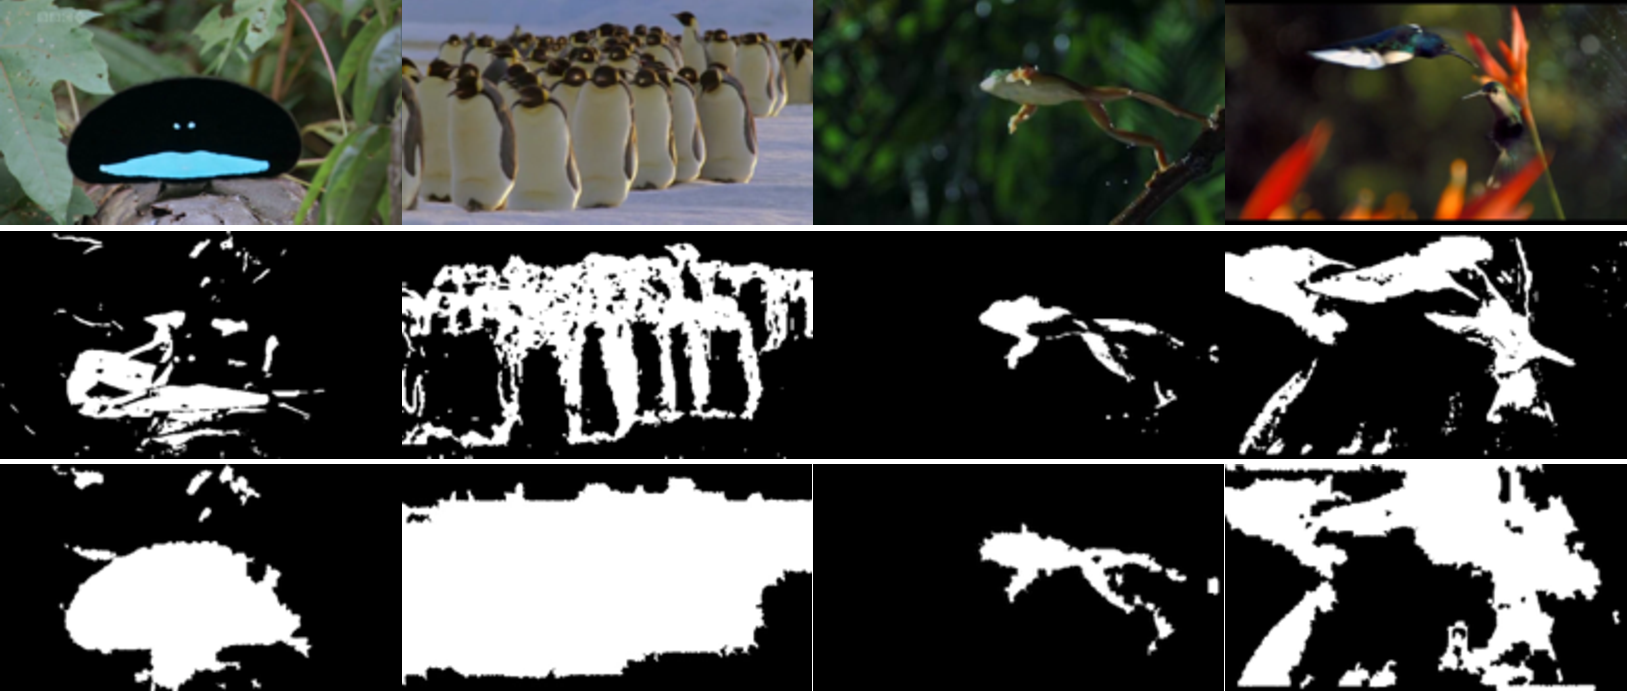
\includegraphics[width=0.97\textwidth]{figures/bs_vs_mask.pdf}
	\caption{Background subtraction masks vs. final masks. The first row demonstrates the original frames, the second row shows the masks generated by background subtraction methods, while the third row is the final masks produced by our method.} 
	\label{fig-bs-vs-mask}
\end{figure*}

We explored the effects of color spaces and different values of $\sigma$ in Equation~\ref{equ-rbf}. We perform the tests on the frog video.
% from SegTrack v2 dataset~\cite{f-li2013}. 
Figure~\ref{fig:sigma} shows the results of three color spaces and different values of $\sigma$. The advantage of one color space over others is not obvious. However, the values of $\sigma$ have an impact on mask quality, reaching a peak at a specific value indicating the appropriate amount of smoothing. In other experiments of this paper, we use the RGB color space and set $\sigma$ to $0.006$.

\begin{figure}
	\centering
	\subfigure[]{\label{fig:sigma} 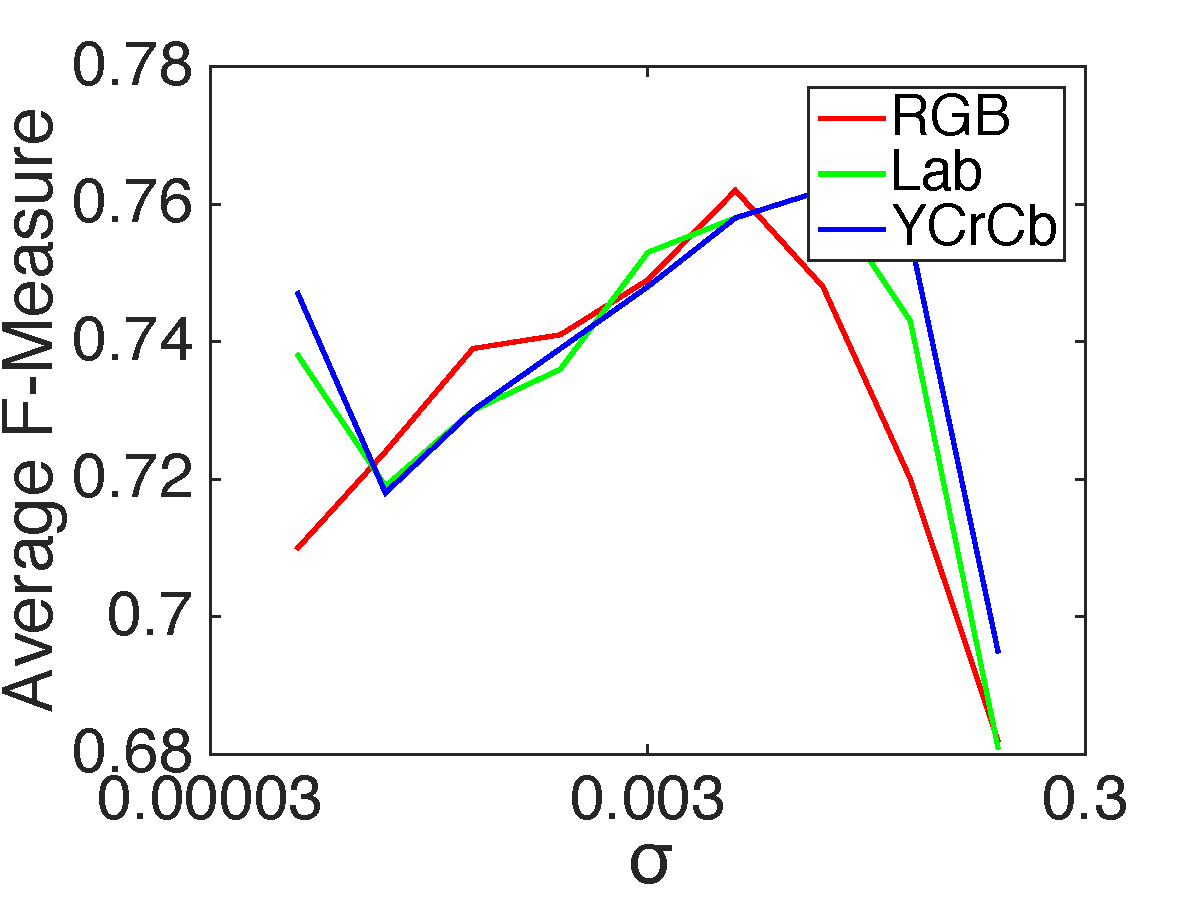
\includegraphics[width=1.65in]{figures/color-space-sigma.pdf}}
	\subfigure[]{\label{fig:constraints} 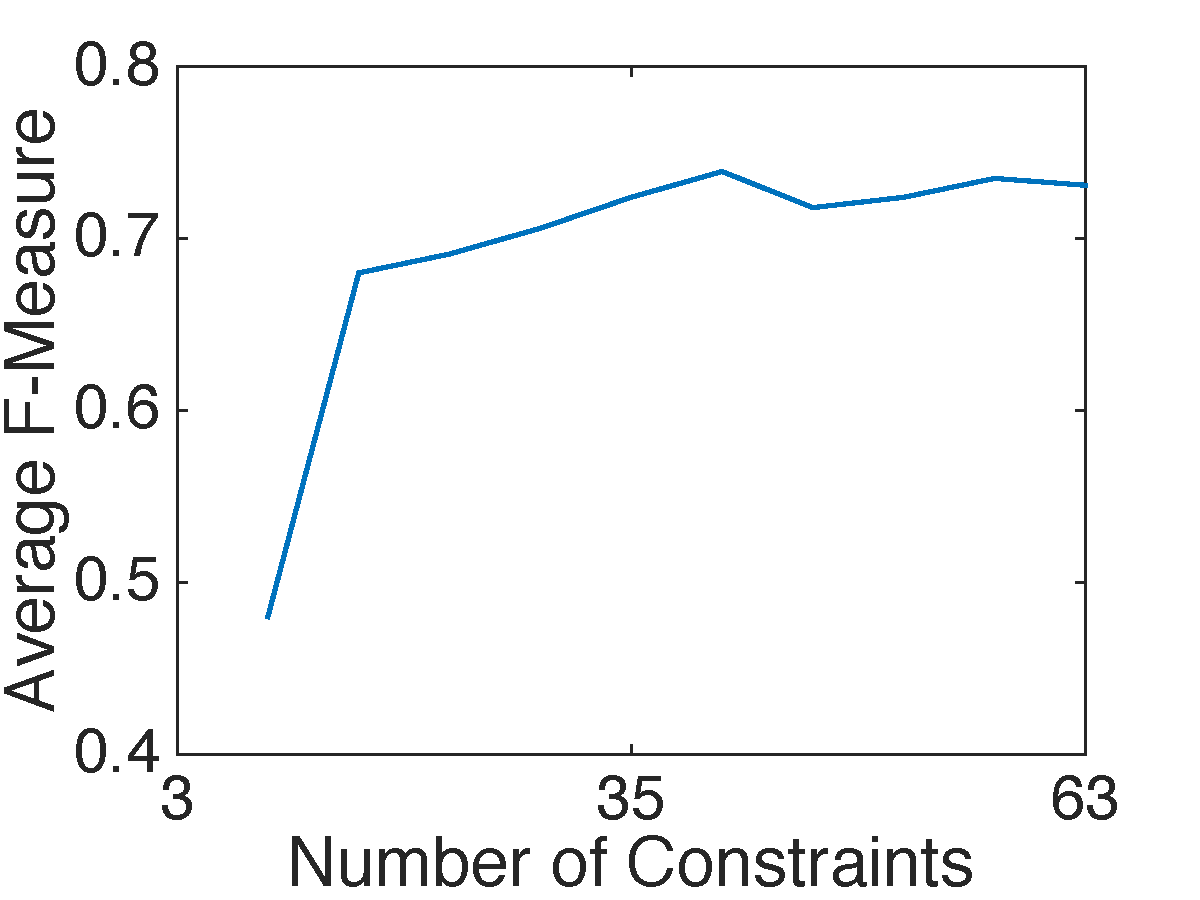
\includegraphics[width=1.65in]{figures/number_of_constraints.pdf}}
	\caption{Parameter Influence:~\ref{fig:sigma} $\sigma$ vs. F-Measure in color spaces RGB, Lab and YCrCb. ~\ref{fig:constraints} Effect of the number of constraints on mask quality. We evaluated the quality of the produced masks using the average F-Measure of the frames with different values of $\sigma$ and number of constraints.} 
%Other parameters are the same for all experiments. Three color spaces are examined, i.e. RGB, Lab and YCrCb, shown as red, green and blue, respectively.}
	\label{fig-params}
\end{figure}

When constructing the RBF, one important parameter is the number of constraints, i.e. the number of terms in Equation~\ref{equ-rbf-ef}.
%, which is used to solve the coefficients in \ref{equ-rbf}. 
As shown in Figure~\ref{fig:constraints}, the number of constraints impacts the mask quality. In this experiment, we set the number of Gaussians to 7, i.e. $|B|=7$. The number of constraints, i.e. $|E|$, is shown along the X-axis in
Figure~\ref{fig:constraints}.
% When $|E|=3$, it is even less than the number of Gaussians, thus the RBF is poorly solved. 
From $|E|=7$ to $|E|=35$, the quality of masks increases with the number of constraints. If we continue to increase $|E|$, there is no obvious benefit. Usually, we set $|E|$ as 2 to 5 times larger than $|B|$.

\section{Content-Aware Video Compression}
\label{sec:vos:cavc}

Video compression standards such as H.264/AVC compress videos as a whole. We applied the approach described above to conduct content-aware compression. We first extract the moving objects and blur the background using a bilateral filter. In this way, we obtain frames with original objects and blurred background. Then we use the obtained video as the input to a H.264 encoder. This method is effective in reducing the bitrate of compressed videos with the same encoding parameters since the blurred background has reduced high frequency components.
% than natual images~\cite{zhu2008}. 
The proposed content-aware compression shares some ideas with the block-based layered approach by Wang et al.~\cite{wang2012} and the sparsity decompression of Chen et al.~\cite{Chen2015}. Our approach is also related to seam carving for compression as proposed by Decombas et al.~\cite{decombas2012}.

\begin{figure*}
	\centering
	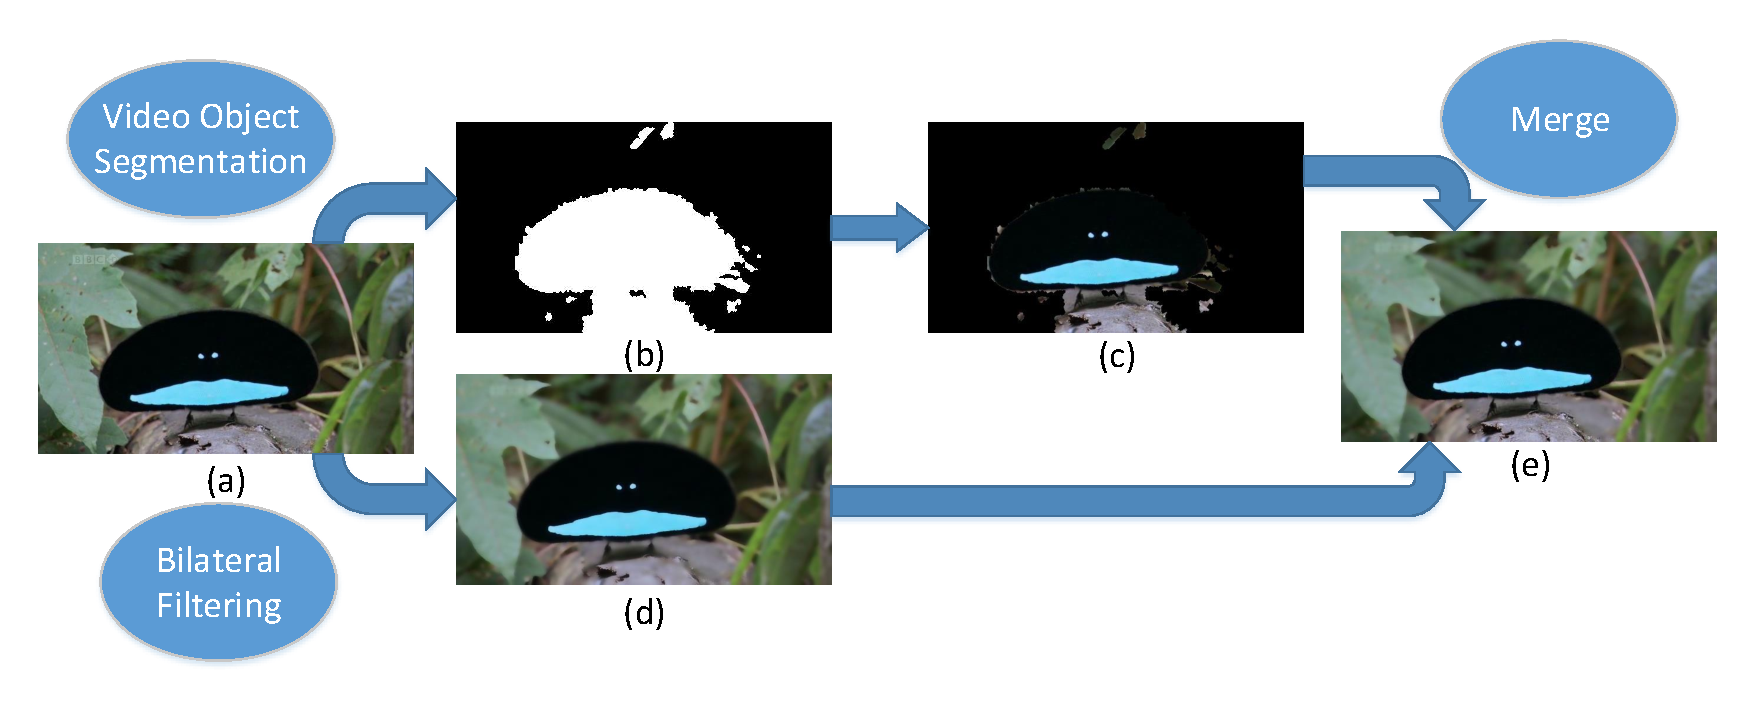
\includegraphics[width=0.97\textwidth]{figures/compression_workflow.pdf}
	\caption{Content-Aware Video Compression. (a) Original frame. (b) Mask generated with the video object segmentation method described above. (c) The object pixels covered by the mask. (d) The frame blurred with bilateral filter. (e) The merged frame.} 
	\label{fig-comp-wf}
\end{figure*}

Figure~\ref{fig-comp-wf} demonstrates the workflow of content-aware video compression. First, a mask (b) of foreground objects is generated with our video object segmentation method, followed by extraction of foreground pixels (c) covered by the mask. The original frame (a) is also blurred with the bilateral filter (d). Finally, the blurred image and the foreground regions are merged together (e). The composite frames are used as the inputs of a typical video encoder such as H.264/AVC. Our results demonstrate that this method can reduce the bitrate of compressed videos.

\begin{figure}
	\centering
	\subfigure[Inter-coding]{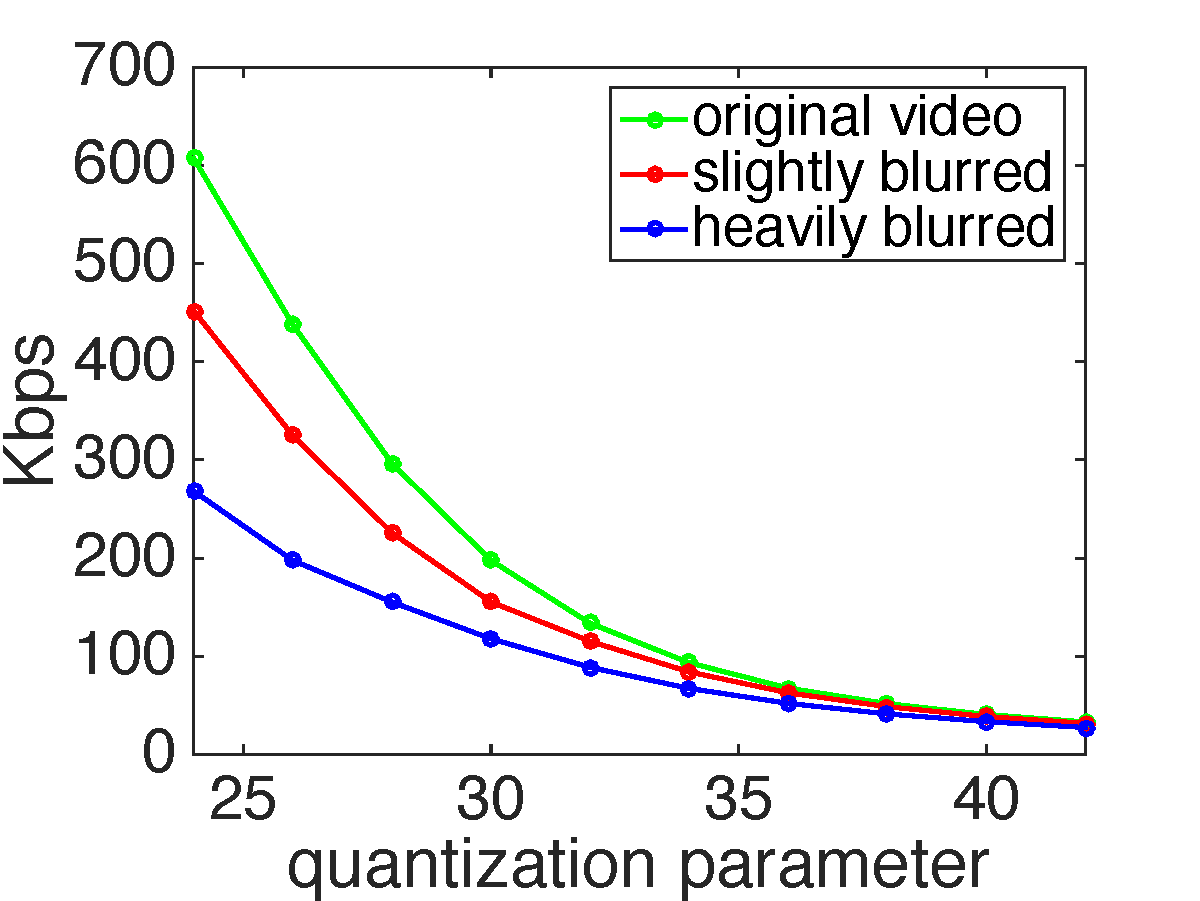
\includegraphics[width=1.65in]{figures/inter.pdf}}
	\subfigure[Intra-coding]{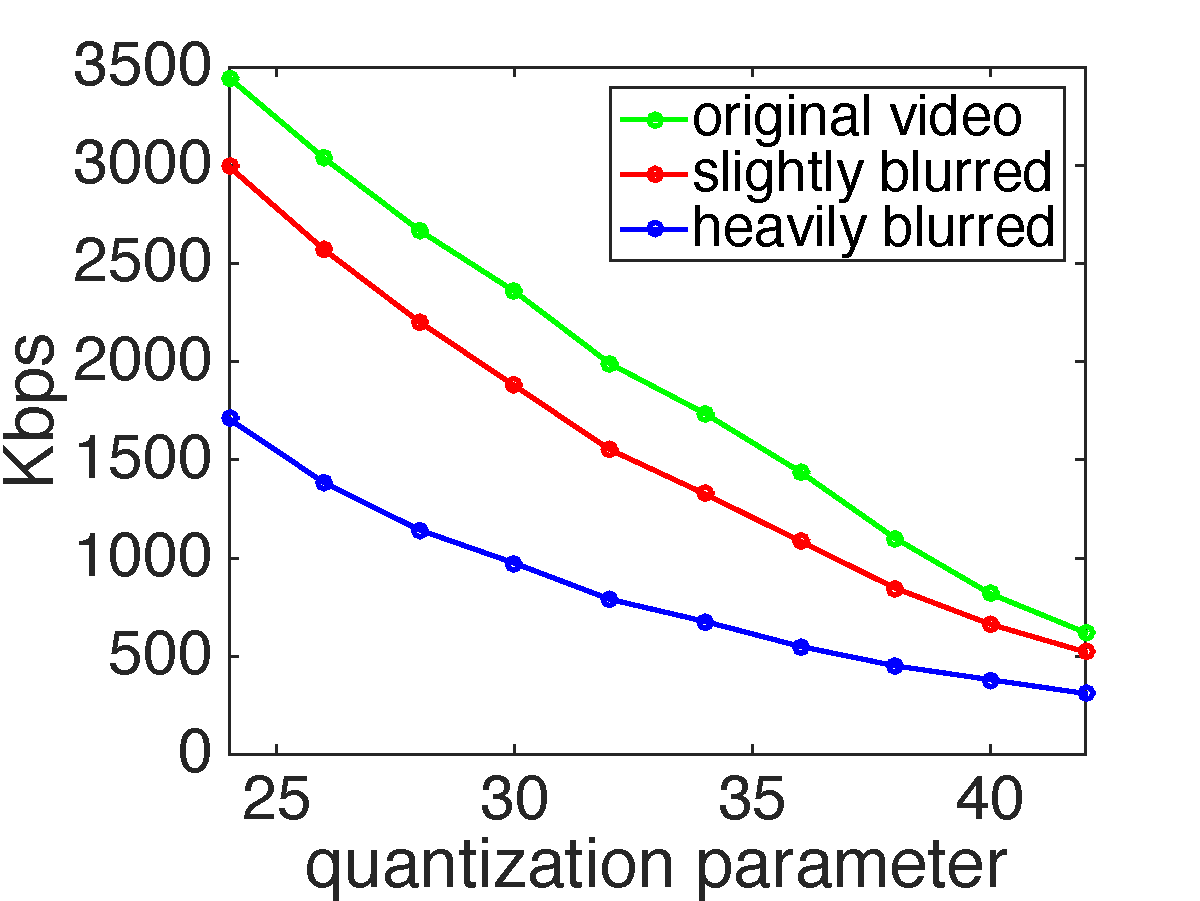
\includegraphics[width=1.65in]{figures/intra.pdf}}
	\caption{Bitrate of Compressed Videos. The X-axis shows the various quantization parameters, while the Y-axis is the bitrate (Kbps) of the compressed videos. The green lines are the bitrate of the original video, the red lines show the bitrate of the composite videos with slight blurring, and the blue lines demonstrate the bitrate of the composition videos but with heavy blurring. (a) and (b) show the results with different coding methods.} 
	\label{fig-comp-br}
\end{figure}

Figure~\ref{fig-comp-br} shows the effectiveness of our video compression method. Figure~\ref{fig-comp-br}(a) shows the results with H.264 inter-coding, while Figure~\ref{fig-comp-br}(b) demonstrates the results with H.264 intra-coding. The green lines illustrate the bitrate of the original video compressed by H.264, which has the highest bitrate among all three types of videos. The red lines show the composite video blurred with the bilateral filter and smoothing parameter set to $0.1$. The composite video achieves a lower bitrate than the original video. Moreover, with lower H.264 quantization parameters, the effectiveness of bitrate reduction becomes more noticeable. We also noticed that the bitrate reduction is higher with inter-coding than intra-coding, since background blurring benefits not only intra-frame compression, but also the prediction between frames. We also tried to increase the smoothing parameter of the bilateral filter, which gives a heavier blurring effect. The blue lines demonstrate the bitrate of the heavily blurred videos. For the inter-coding, the bitrate is slightly reduced, while for the intra-coding, the bitrate reduction is more obvious. We conclude that compression of videos with high-resolution foreground and blurred background can effectively reduce the bitrate, the quantity of reduction depends on the blurring degree of background, and the effectiveness is more noticeable with inter-coding than intra-coding.
